%!TEX root =  main.tex
\chapter{Proof of concept}\label{chapter:Implementation}
%
In this chapter, more details are going to be given about the framework implemented based on the formal model and architecture specification given in the previous chapter.

Section~\ref{sec:framework} discusses framework architecture, and system implementation details, and framework limits. Section~\ref{sec:framework_operations} presents implementation details about framework operations. Section~\ref{sec:app} describes few possible senarios and applications that could utilize micro-clouds platform. In Section~\ref{sec:results} presents results of our experiments.
%
%
\section{Platform implementation}\label{sec:framework}
%
In this section, we are going to introduce an implemented proof-of-concept framework based on the model proposed in the previous chapter~\ref{chapter:Micro_clouds}. The framework is called \textbf{Constellations} or \textbf{c12s}\footnote{https://github.com/c12s} for short because it is strongly influenced by nature and the neverending number of galaxies that the universe is (not only) composed of. Similarly, we are trying to create a universe of clusters that will serve humanity to help them with their day-to-day tasks. The framework is \textbf{open-source}, and it is implemented using the microservice architecture with services that have distinct role and purpose to the entire system. These services are:

\begin{itemize}
	\item \textbf{Gateway}, this purpose is to export services feature to the rest of the world. Gateway is designed as a REST service, accepting $JSON$ style messages, so that various clients can communicate to the system. When the request arrives at the gateway, if the request is valid it will pass the request to the rest of the system. It communicates to the rest of the services to check if the user exists, if he / she has proper rights for actions he / she sends, and if not, returns the proper message and and does not propagate it to the rest of the system.
	\item \textbf{Authentification \& Authorization}, the sole purpose of this service is to store users and their credentials. This service will validate does user exists in the system, and does he have certain rights to perform some specific operation. Users that often use the system will be stored in the cache layer of the service so that on the next request his actions are done faster. Users that do not use the system that often will not be stored in the cache, until the first use. After that, if the user does not use the system for some time, he/she will expire from the cache.
	\item \textbf{Queues}, the purpose of this service is to prevent huge request load to the system and to accept more user requests. When the user submits any \textbf{mutation} operation -- an operation that changes the state of the system, these operations will be put in the queue. User can create their queues, to prevent long lines for specific tasks. For example, users can create queues for specific tasks, and use them only for those tasks, while other queues could be general-purpose queues. On system start, every user will start with one queue --- \textbf{default}. When doing mutations on different parts of the system, the user can specify in metadata which queue he wants the task to go to. This service implements a token bucket rate-limiting algorithm~\cite{MathewsKG17} to prevent congestion of the system.
	\item \textbf{Nodes}, this service stores and maintains pieces of information about registered nodes in the system. All node hardware and software details will be stored in this here. This service is also responsible for storing metrics data, accept health-check requests from nodes, and inform the rest of the system that the used node is alive.
	\item \textbf{State}, is the heart of the system. This service stores all information about architecture, clusters, regions, and topologies. When a new cluster/region/topology is created, this service will setup watchers for nodes, so that if the node does not send the health-check signal for some time, that node will be declared dead. This is important so that at any moment we must know the state of the clusters and their utilization. This service as well will cache frequently used nodes data, so that on the next request node lookup is faster, since we can have a huge number of nodes, topologies, clusters and pieces of information about them. To prevent data loss, this service will first store a copy of the operation before attempting any mutation of the system.
	\item \textbf{Log}, is responsible for storing all log and trace data from every service. Here a user can check whether all jobs are done, whether there is some error and possibly why the error happened to resolve it or fix it for the next time. From a user point of view, this is \textbf{read only} service and from a system view, this is \textbf{write only} service.
	\item \textbf{Command push}, the purpose of this service is to push commands and operations to the nodes user desired. This service implements a token bucket rate-limiting algorithm~\cite{MathewsKG17} to prevent constant data push to the nodes. Similar to the state service, this service will store a copy of operation information locally before attempting any push to the nodes. This information will be deleted, once the operation reaches all decided nodes and all of the responses with the acknowledge (ACK) message.
\end{itemize}

\noindent
All services are highly customizable and all have their configuration file that could be changed and adopted. All these services are easy to extend to support new operations and pieces of information about nodes, regions, clusters, topologies, and latter on applications, configurations, namespaces, etc. 

The system operates with four commands, where three of them follow formal models described in the previous chapter. The last command is a simple command to list logs for every user.

Regarding~\ref{sec:access_pattern}, the framework operates as a master process is running in Kubernetes, and through that process, all commands are issued. Future applications can communicate with nodes as stated in~\ref{sec:application_model}. They do not require communication with the master process at all, they can communicate with the formed cluster using topics and streams.

In the rest of this section, we will see details about all operations, as well as used technologies to implement the whole system. Possible applications and future directions for application development will also be described. System architecture is shown in Figure~\ref{fig:fig11}.

\begin{figure}[H]
	\begin{center}
		\includegraphics[scale=0.7]{images/FIG5}
	\end{center}
	\vspace{-0.5cm}
	\caption{Proof of concept implemented system.}
	\label{fig:fig11}
\end{figure}
%
%
\subsection{Technologies}\label{sec:technologies}
%
All services are implemented using the Go\footnote{https://golang.org/} programming language, because of its well-known tooling, support for developing system software, web-based applications, small binaries but also, great concurrency model, and ability to build binaries for almost any architecture without any code changes. All services rely on Go implicit \emph{interface} implementation mechanism. Every technology or component used in the system can be swapped for some other, as long as that component implements \emph{interface} fully. The framework is developed in such a way that is relatively easy to extend, or switch and use different components and technologies.

As the main storage layer for our system, we used etcd\footnote{https://etcd.io/}, a popular open-source key-value database, that shows good performance, and it is mostly used for configuration data. Metrics data are stored in the open-source time-series database InfluxDB\footnote{https://www.influxdata.com/}. 

Communication between microservices is implemented in RPC manner using gRPC\footnote{https://grpc.io/}, and Protobuf\footnote{https://developers.google.com/protocol-buffers} as a message definition. gRPC and Protobuf are open-source tools designed by Google to be scalable, interoperable, and available for general purposes. Communication between nodes and the system is carried out using NATS, an open-source messaging system. Health checking and action push to nodes are implemented over NATS\footnote{https://nats.io/} in a publish-subscribe manner.

Caching layer for every service is implemented using Redis\footnote{https://redis.io/} key-value, in-memory database. It is important to notice, that all concrete tools that are used, are easily swappable for some other as long as they implement a proper interface.

All communication with the outside world is done in a REST manner using JSON encoded messages over HTTP. To communicate with the platform, we have developed a simple command-line interface (CLI) application also using the Go programming language that sends JSON encoded messages over HTTP to the system.

Every service is packed in a container, and for this purpose Docker\footnote{https://www.docker.com/} containers are used. To achieve automatic orchestration, and self-heal, and up-time, all services that are packed in containers, are running inside Kubernetes.

Every service will log details about its usage and calls, as well as traces how requests are going. Log data is stored outside the service and container, and pieces of information will be sent to centralized log storage on every $t$ seconds specified by the user. Sending intervals could be changed and adapted using the configuration file for every service independently.

Log data will be stored in the two levels:

\begin{enumerate}[start=1,label={(\bfseries \arabic*)}]
	\item \textbf{system level}, this data is generated by the system and could be viewed by administrators of the system \textbf{only}. Operations people in the team (eg. DevOps or SREs), and developers cannot see it, but providers can.
	\item \textbf{user level} that stores information about user requests that \textbf{only} users can see. This type of data will not be visible to the developers of the system, and only users that created these logs will be able to see them.
\end{enumerate}

\noindent
Log storage could be searched to see the general state of the system, and pieces of information about user requests and the state of their requests.
%
%
\subsection{Node daemon}\label{sec:node_daemon}
%
Every node runs a simple daemon program implemented using the Go programming language, as an actor system (Ref. secion~\ref{sec:actor_model}). The actor system is developed for this purpose. When a message arrives, the proper actor will react based on the message type, or discard it if the type is not supported. 

Extending such a system is rather easy because users need to simply write a new actor and logic that goes with them and register it to the system.

When the daemon start, it will first read the configuration file to do the proper setup and then will contact the actor system to start all the actors. 

System messages will be sent to the daemon, but it will not react to these messages. Daemon is not able to communicate with any actor directly. All communication goes through the actor system which is responsible to pass messages to the actors. The actor system at this point has only four existing actors:

\begin{enumerate}[start=1,label={(\bfseries \arabic*)}]
	\item \textbf{cluster actor}, this actor reacts on messages about new cluster formation, but he is also responsabile to contact rest of the system that message has arrived.
	\item \textbf{internal actor}, this actor react to messages from other actors to update the daemon state. For example, on new cluster creation, this actor will update daemon id, name, labels, etc.
	\item \textbf{health actor}, this actor will periodically send \emph{health-check} data to the system about node state, utilization, etc. This actor will communicate to the rest of the hardware to get proper pieces of information, to collect logs from the node, and send all that data to the system.
	\item \textbf{gossip actor}, this actor will communicate with other peers in the group using SWIM protocol techniques.
\end{enumerate}

\noindent
The actor system will monitor these actors, and in case any of the crushes, the actor system will restart them. 

Listing~\ref{lst:listing3} show the actor system hierarchy of existing actors.

\lstinputlisting[caption={Actor system hierarchy.}, label={lst:listing3}, captionpos=b, xleftmargin=.35\textwidth]{listings/listing3.txt}

\noindent
Before daemon starts, the user needs to specify some parameters for proper configuration like: 

\begin{enumerate}[start=1,label={(\bfseries \arabic*)}] \label{imp:features}
	\item \textbf{identifier}, represents unique identifier of the node. When a node is not a part of some cluster, this can be whatever the user wants. Once the node is a part of some cluster, the identifier will be updated, and it is not advised to change it manually afterwards.
	\item \textbf{name}, represent name of the node. This property also can be changed when a node is part of the cluster, otherwise, it can be whatever we want.
	\item \textbf{labels} represent the specific features of the node. Labels are used to query for free nodes, and there is no formal restriction of what they can or can not be. This property can be changed when the node is a part of some cluster. It is advised that as labels we put some specific features of the node that might be beneficial for the user who is looking for nodes to create new cluster/s.
	\item \textbf{health-check details}, here we have pieces of information to control the health-check mechanism. Since nodes communicate with the rest of the system via publish-subscribe events, we must specify the address of the rest of the system and the topic name, where we publish our pieces of information.
	\item \textbf{system information}, represents basic information for a node to know how to contact the rest of the system. We should specify the system address, so that node knows where to send messages, and where are messages are coming from. We can also specify the version of the system we are trying to contact. System version could be used to support \textbf{backward compatibility} if we have multiple API versions of the system running at the same time or some period.
\end{enumerate} 

\noindent
Configuration can be done easily using the YAML configuration file. 

Listing~\ref{lst:listing1} shows simple YAML configuration file for daemon process.

\lstinputlisting[caption={Daemon configiration file}, label={lst:listing1}, captionpos=b, xleftmargin=.35\textwidth]{listings/listing1.yaml}

\noindent
Based on the configuration file, the daemon will start a background health-check mechanism, and it will subscribe to the system, using an identifier as a subscription topic. The background thread will contact the system repeatedly using a contact interval time, specified in the configuration file. 

On every health-check, the node will send labels, names, IDs, and metrics to the system (e.g., CPU utilization, total, used, free ram or disk, etc.). The specified labels will be used when the user is querying for available nodes, while the node id will be used for reservation when forming a cluster.

At the first start of the daemon, when the node is free, the user can specify whatever node id he/she wants. Once, the node is a part of the cluster, the node id will be updated to match that. Node id update will happen on the cluster formation process.
%
%
\subsection{Separation of concerns}\label{sec:framework_SoC}
%
IThe implemented framework follow the clear SoC model, presented in~\ref{sec:separation_of_concerns}. Since the presented model consists of three components, the implemented framework is deals only with \textbf{resources}~\ref{soc:resources} part of the SoC. 

Its job is to organize nodes into clusters, regions, and topologies, to make them communicate and expose their resources to the upper layer of SoC for utilization. The upper layer will run services on these resources, to collect data from data creators and process them as requested.

The upper layer must have set up the infrastructure to do any processing or storage. This middle layer is the binding element between the layers.
%
%
\subsection{Transactions}\label{sec:transaction}
%
Current implementation follows the saga pattern (cf.~page~\pageref{sec:sagas}) for transactions, and isolation is added using semantic lock by adding states to the task. The task can be in one of following states: $(1)$ PENDING, $(2)$ IN PROGRESS, $(3)$ CREATED, and $(4)$ FAILD. 

Until the task reaches \emph{Created} state, no other operation can be done on that cluster configuration.

The cluster formation transaction is split into a few sub-transactions: $(1)$ reserving nodes, $(2)$ writing cluster information, and $(3)$ sending cluster information to push service and ultimately sending pieces of information to the nodes. 

The rollback mechanism is implemented using \emph{choreography}, and communication between the various services is done asynchronously using message queues.
%
%
\subsection{Garbage collection}\label{sec:gc}
%
The current garbage collection process is pretty trivial since there is no complicated graph of items connected to the cluster information details.

The process will scan tasks with the state \emph{FAILD} in the background, and it will remove those items. Related details to the cluster information, for example, node metrics, will expire automatically since there is a lease attached to them.

Another resource that will be automatically deleted is node data. If a node health-check message does not reach the system in some time, the node lease will expire and data will be removed automatically.
%
%
\subsection{Limitations}\label{sec:framework_limits}
% 
The framework at the current state has some limitations that we \textbf{must address}. As shown in figure~\ref{fig:fig11}, for purpose of testing the system, and to give the users any way to interact with the system, a CLI application is implemented. This is a good option for initiating commands to the system. The problem with this approach is that showing logs, and topologies might be limiting the users, especially if they monitor and supervise multiple topologies with regions and clusters.

For monitoring, a tool with UI would be a better solution and it can show more details. For a small amount of data, when topologies are relatively small, CLI could be used. But for some real-world applications, desktop, and/or web-based UI will be a much better solution, and CLI can be used for fast lookup on specific pieces of information about clusters and nodes, for example.

The current implementation of the queueing system is \textbf{limiting} because if we want to extend the system with new queues we need to shut down the whole service, and that is not the best solution. But since the goal of this thesis is not queue management, but micro-cloud formation, protocols, and formal modeling.

Since the goal of this thesis is not queue management, and the purpose of this thesis is not Human-computer interaction, but micro-cloud formation, protocols, and formal modeling, mentioned limitations should be the topic of the future work~\ref{sec:future_work} section.

The current implementation do not include garbage collection of connected dependent items, and users cannot influence garbage collection decisions. This should be one of the topic of the future work~\ref{sec:future_work} section as well.
%
%
\section{Operations}\label{sec:framework_operations}
%
In this section, we are going to describe all implemented operations in the framework and present specific details about every individual operation.
%
%
\subsection{Query}\label{sec:query} 
% 
The query operation is used to show all free nodes or filtered free nodes that are registered into the system, to the user (yellow arrows in Figure~\ref{fig:fig11}.). 

When a user wants to get information about free nodes, they need to submit a \textbf{selector} value which is composed of multiple \textbf{key-value} pairs.  These key-value pairs can be any alphanumeric set of symbols for both keys and values. Based on that key-value pair the system will do the query of the free nodes.

The selector will be used as a search mechanism to compare the labels of every free node that exists in the system. The nodes that are satisfying the rules~\ref{frm:query_rule} defined in Section~\ref{sec:cluster_formation_protocol} will be present in the result.

This operation is done before the formation of new topologies, regions, or clusters --- mutation of the system. The user first needs to get a list of free nodes, then he can choose nodes that are best suited for him and try to form topologies, regions, or clusters of them.

The querying process is a little bit changed from one presented in Section~\ref{sec:cluster_formation_protocol}. The only change that is made is the addition of the \emph{Gateway} service that will pass requests into the system and prevent overflow of requests. This change \textbf{does not} affect or validate the formal model presented before, since the added service does not interfere with the process of searching nodes or changes to the system.

Figure~\ref{fig:fig14} shows a communication diagram for the query action, with the addition of the Gateway service.

\begin{figure}[H]
	\begin{center}
		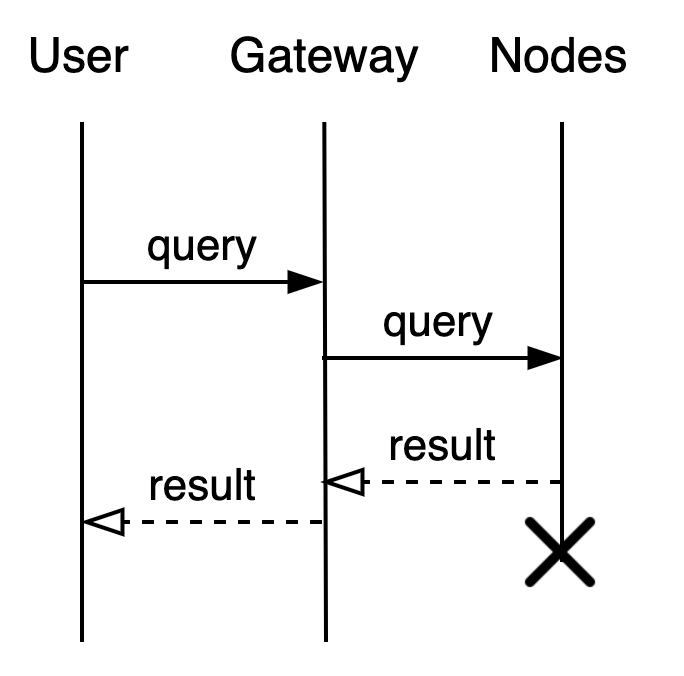
\includegraphics[scale=1]{images/Figure14}
	\end{center}
	\vspace{-0.7cm}
	\caption{Low level communication protocol diagram of query operation.}
	\label{fig:fig14}
\end{figure}

\noindent
Query operation is implemented using \emph{api composition} pattern (cf.~page~\pageref{par:composition}).
%
%
\subsection{Mutate}\label{sec:mutate} 
%
Mutate operation (orange arrows in Figure~\ref{fig:fig11}.) changes the system state by creating, editing, or deleting clusters, regions, and topologies. When a user wants to perform a mutation over the system, the desired state needs to be specified \textbf{declaratively} using a YAML file and submitted to the system. When the state is submitted, the system will do the rest of the job to ensure that the state desired by the user is reached.

The users specify which nodes are forming the cluster. Optionally, users can also specify labels and names on the node level, and retention period on the cluster level. The retention period is used to describe how long metrics are going to be kept. When the retention period expires, the metrics data will be deleted or moved to another location. 

When forming a topology, users can assign a name and label to the entire topology. These parameters will be used when the user wants to query all topologies to get full information about regions, clusters, and nodes inside a topology.

Mutate operation is \textbf{immutable}, which mean that there will be no in-place changes to the existing state. If a user wants to do any update, he/she needs to specify a full new state that will replace the existing one. This operation is \textbf{atomic} as well, which mean that a whole new state must be able to replace the existing state. If this happens, the system will replace the old state with the new one. The main storage that stores configuration data is a key-value store implemented using an etcd database. The key that will be used to store the configuration data is the whole path of topology, regions, cluster, node, while the value represents the state desired by the user. 

Listing~\ref{lst:listing4} shows structure for key-value pair that is stored in the main database, where on top we can see a structure of the \textbf{key}, and below it we can see the structure of the \textbf{value}. This kind of structure is similar to OS file-system data organizations of files and folders.

\lstinputlisting[caption={Structure of stored key-value element.}, label={lst:listing4}, captionpos=b, xleftmargin=.25\textwidth]{listings/listing4.txt}

\noindent
We store as well one additional information about labels \textbf{index} value. This index is used for a faster query of elements when doing labels comparison. To find elements we can query in a similar way like searching files and folder structure. The etcd in newer version \textbf{do not allow} hierarchical keyspace, but what they allow is \textbf{ranged} query by some \textbf{prefix}. This is useful as well because we can still get all regions in topology, clusters in the region, or nodes in the cluster if we know to which group they belong.

Mutate operation is not idempotent by nature, but the whole process behind it makes mutate an idempotent operation. Whether the user tries to create already existing infrastructure by changing the order of regions, clusters, or labels in the nodes, or if he for whatever reason did not get confirmation that infrastructure is created, an existing infrastructure will not be created. This is done in such a way, that $State$ service (Figure~\ref{fig:fig11}) will keep the information set about created infrastructure. This information is implemented as a \textbf{flat keyspace} set, that have information. On every mutation request, the system will test if such a topology already exists. If such topology already exists, the user will get confirmation that his infrastructure is created. If such topology do not exist, a new cluster formation protocol~\ref{sec:cluster_formation_protocol} will be initiated. The mutation confirmation is followed by a \textbf{unique id}, which the user can use to query steps, logs, and traces that are done in process of working towards the state desired by the user. Logs service can give the user complete details about his task state using that unique id.

When creating topologies, the user is free to give whatever name he wants for every region, cluster, and node. The only restriction is that name should be the alphanumeric set of characters. Listing~\ref{lst:listing2} shows an example of a user-defined state that forms the topology of one region with one cluster that contains three nodes, with a retention period of 24 hours. The whole topology will have the same set of labels, but $node3$ redefines this rule by specifying its own.

\lstinputlisting[caption=Example of mutate file using YAML., label={lst:listing2}, captionpos=b, xleftmargin=.3\textwidth]{listings/listing2.yaml}

\noindent
After all, nodes that should form a cluster, acknowledge cluster formation message, they will inform the system that the message is received, and they will start the process of cluster formation. This process is done by using SWIM~\cite{DasGM02}, a Gossip style protocol. When every node has a complete list of its peers that should be in the cluster, the process of cluster formation is done. 

On the next health-check message, every node will send its \textbf{id} that is telling the system that he is part of some cluster. This kind of messages will be used in the $State$ service to validate that cluster is alive and well, or that some nodes (or all), are dead or down if \textbf{id} is not received. 

Gossip style protocols (like SWIM) could be used in the future to propagate information in the cluster, without explicitly ping every node in the cluster.
%
%
\subsection{Queueing}\label{sec:queueing}
%
When doing mutation, users can target a specific system queue, by adding a metadata part in the configuration file. With this ability, users can aim for specific queues just for the mutation to avoid long waiting times if other queues are full. Currently, the system does not have any limitations, restrictions, or logic that will specify which queues are used for what or give them special rules or permissions. This can be viewed as a \say{gentleman agreement}, that in one team, operations users can proclaim specific queues like \textit{mutatation} queues used maybe for specific topologies, and later on for other operations as well.

The queue service starts only when the $default$ queue exists. Adding a new queue to the system is implemented using the configuration file, for convenience only. 

Listing~\ref{lst:listing5} shows an example of queue service with two additional queues with specifications of their parameter needed for token bucket operation~\cite{MathewsKG17}. Also, we can see configuration pieces of information for instrumentation of a single service, and the same configuration is implemented for all specified services shown in Figure~\ref{fig:fig11}.

\lstinputlisting[caption={Structure of stored key-value element.}, label={lst:listing5}, captionpos=b, xleftmargin=.25\textwidth]{listings/listing5.txt}
%
%
\subsection{List}\label{sec:list} 
% 
The list command shows the current state of the system for the logged user (blue arrows in Figure~\ref{fig:fig11}.). Logged user is able \textbf{only} to see infrastructure he/she has created or maintains. All other infrastructures, created by other users, will not be visible to the users that are not creators or maintainers.

To view his/her infrastructures, the user can specify what part of the system he/she wants to see using a set of labels or list of key-value pairs, which will be used by the system to determine what the user wants to see. This process is similar to \textbf{selector} shown in the query~\ref{sec:query} operation. 

There are two levels of details that user can specify:

\begin{enumerate}[start=1,label={(\bfseries \arabic*)}]
	\item \textbf{global view}  of the syste, or all topologies he/she manages with just basic information like resource utilization, number of regions clusters and nodes.
	\item \textbf{detail view}, or details about a single topology (i.e., regions, clusters, and nodes in a single topology). Users can specify a more detailed view of a single cluster, meaning the users will get information about what resources the cluster has, but also resource utilization over time (using stored metrics information) and so on.
\end{enumerate}

\noindent
Both options can be useful if operations people need different details levels for different topologies. List operation is implemented using \emph{api composition} pattern (cf.~page~\pageref{par:composition}).
%
%
\subsection{Logs}\label{sec:logs}
% 
The logs operation shows stored logs and traces to the user (purple arrows in Figure~\ref{fig:fig11}.). Same as previous operations, the user needs to be registered and logged in to be able to perform this action. With this action, the user can see the state of his/her operations and actions. The user can choose between two options for querying his/her logs:

\begin{enumerate}[start=1,label={(\bfseries \arabic*)}]
	\item \textbf{get}, for this option a user needs to provide a unique task id that is given to the user when he/she creates a mutate operation. With this option, the user will get a full list of steps, traces, and logs collected over the time the system was setting up his/her desired state.  
	\item \textbf{list}, with this option user can specify \textbf{selector} using list of key-value pairs in a similar way to query~\ref{sec:query} and mutate~\ref{sec:mutate} to filter only parts of the traces that contain the same labels as selector does.
\end{enumerate}

\noindent
This action is implemented in some basic aspects, as this action can return a huge amount of data that require some better visualization than CLI.
%
%
\section{Results}\label{sec:results}
% 
For the ease of testing, a few ARM-based nodes that are easy to move from place to place have been used. The test should be conducted on the heterogeneous nodes, to see how the system will react to different architectures and resources. In our tests, we have used:

\begin{itemize}
	\item 9 Raspberry Pi 3+ Model B with 1GB LPDDR2 SDRAM, 16GB SDCard storage, and 1.4GHz Cortex-A53 64-bit SoC running Raspbian Linux, a Debian-based operating system.
	\item 3 Beagle bone black devices with 512MB DDR3 RAM, 4GB 8-bit eMMC on-board flash storage, and 1GHz ARM Cortex-A8 running a version of Linux Debian operating system.
\end{itemize}

\noindent
as test heterogeneous nodes for creating clusters, regions, and topologies.
%
%
\subsection{Experiment}\label{sec:experiment}
%
Using Go tooling, we were able to build daemon service without changes and dissiminate on all nodes without problems.

We ran tests on different configurations and different nodes clusters using these nodes. All nodes were connected on the network, and experiments were conducted in a controlled environment. Nodes that should be a part of the same cluster were connected on same network for easier experiments.

Experimental research was realized in the laboratory of the Department of Informatics at the Faculty of Technical Sciences in Novi Sad. The laboratory of the Department of Informatics is equipped with adequate computer, communication and software equipment on which the set goals in this thesis can be fully realized.

Our experiment started with separating nodes into groups of \textbf{three}. This number is chosen because in DS, an odd number is used in cases when we need to reach some agreement and we need major majority like consensus, for example. This is not important for purpose of this thesis, we could pick any number, membership protocol does not makes a difference if there are three or four or eleven nodes in the cluster.

After nodes had been separated, we created a configuration file for every node, setting up default parameters for every property node daemon required~\ref{imp:features}. After all services were up and running, we turned the nodes on, and health-check protocol~\ref{sec:health_check_protocol} started at uprfront defined time, which we had set for test purposes at \emph{1 minute} interval. Logs, resources and other node details were set to \emph{15 seconds} interval, so between health-check intervals, daemon would collect resource information \emph{four times} before sending it to the rest of the system.

For convenient testing, all nodes had the same set of labels, and as labels we chose OS name, OS version, architecture version, node name basic details about resources of the nodes.

After some time, we were able to see all nodes registered in the system. When all nodes had been sending health-check ping for some time, and we had a stable system, we issued a mutate operation creating clusters of nodes that are logicaly close ot each other, and we initiated cluster formation protocol~\ref{sec:cluster_formation_protocol}. After the protocol was done, we ended up with four clusters as we intended. We tried to initiate the same command again to test idempotency check~\ref{sec:idempotency_protocol}, and we got the message that clusters already existed.

To increase capaticity, we extended clusters by creating new ones using \emph{three clusters} with \emph{four nodes}. We created new new mutate file, and initiate new mutate command. After some time, we saw that one cluster was down and that we now had \emph{three clusters} with \emph{four-nodes}, as we intended. After successful creation of new clusters, we dleted down cluster.

The last test was to test health-check protocol once again - we disconnected one random node from the power supply, and since that node ping was missing, the system was able to detect which node was \emph{down}. This concluded our experiment.
%
\section{The existing solutions enhancement}~\label{enhancement_of_the_existing_solutions}
%
The protocols defined in this thesis could serve as a base layer for the system developed from scratch. On top of such a solution, we can add other services and features like scheduling, storage, applications, management, monitoring, etc. The protocols described in this thesis ensure proper node registration into the system, organization, and reorganization of node resources into clusters, regions, and topologies, bringing disposable micro clouds closer to the users at the network edge, allowing that requests are served from the local micro cloud.

The existing orchestrator engines (e.g., Kubernetes, Apache Mesos, Docker Swarm, etc.) operate one cluster level~\cite{BurnsGOBW16, VermaPKOTW15, RossiCPN20, KubeEdge, KubeMulti}. The single cluster could span over multiple availability zones in the cloud, minimizing the chance that a failure in one zone impairs services in other zones~\cite{KubeMulti}. Kubernetes allow extension in terms of multi-cluster deployments~{\cite{KubeMulti}}. In such a scenario, Kubernetes is handling these clusters as disposable --- "treating \textbf{clusters} as cattle, not pets" (i.e., numerous servers/clusters built using automated tools designed for failure, where no servers/clusters are irreplaceable~\cite{CERN}).

The model proposed in this thesis goes one step further, allowing the creation of disposable micro clouds. Such an extension allows infrastructure optimization in more dimensions~\cite{ForestieroMMPS14}. The users are allowed to build numerous micro clouds designed for failure using automated tools where no micro cloud is irreplaceable --- "treating \textbf{micro clouds} as cattle, not pets."

The existing solutions can integrate the model proposed in this thesis to serve as a node register. Such integration allows the registration of new nodes into the system, allowing the existing orchestration engines to use new nodes, and expand their available resource pool. In form of specification, the users can provide a list of which available EC nodes need to be part of some micro cloud. The system will communicate with the existing orchestrator agent to register/unregister them with the existing cluster. In such a scenario, we can hook on the existing orchestrator health-check mechanism informing our system that a node in some cluster is alive. Unused nodes still use the health-check protocol defined in this thesis informing the system that they are still available for utilization.

The proposed model preserves the node's topology allowing cloud providers and orchestrator engines to treat micro clouds disposable, abstracting infrastructure to the level of software --- infrastructure as software~{\cite{Fitzgerald}}. This approach benefits from the already available tools, principles, and techniques (e.g., reuse, testing, modeling, and evaluation). The already available tools can be used for the disposable micro cloud infrastructure definitions.

The model developed in this thesis is not competing with the existing orchestrator tools. It is not orchestrating applications, but it is a free nodes register and micro clouds infrastructure descriptor allowed to be offered as a stand-alone service bringing disposable micro clouds model to the users. The model allows integration with the existing orchestration tools, leveraging existing mechanisms and best practices. Cloud providers can create an operator for various orchestration engines. This allows them to offer dynamically created, disposable micro clouds as a service to their users, using infrastructure as software principles.
%
%
\section{Applications}\label{sec:app}
%
This research focuses on a platform with geo-distributed edge nodes that can be organized dynamically into the micro data-centers and regions based on the cloud model, but adapted for a different environment. This middle layer helps the power-hungry servers reduce traffic by serving the nearby population requests. Users are getting a new platform as a blank canvas, and there is no limitation in what applications they can develop. Integrating hardware and/or software, even more, connecting sensors and things around us and eventually an operating system that will be capable of running city/state infrastructure without human intervention.

The main advance of EC, when compared to the cloud-only approach, is the acceleration of the communication speed. The cloud could bring huge latency, while EC originates from peer to peer systems~\cite{LopezMEDHIBFR15}, serving only local population needs, minimizing potentially huge round-trip time of the cloud. Furthermore, presented model expands peer to peer systems into new directions and blends them with the cloud to allow novel human-centered applications. 

If we imagine that we put sensors on a specific group of users and/or places in the city/state and monitor them in real-time, we can process these streams of data directly close to where they are, where they are moving and going. We could monitor air pollution for example, and make decisions in real-time to suggest users not to walk in some area, especially if they have some known respiratory problem.

Geo-distributed nodes represent a great idea to do any kinda monitoring and processing especially for natural phenomenons and do alert as soon as probes, sensors, or other things detect even the slightest changes. For applications like self-driving cars, delivery drones, or power balancing in electric grids require real-time processing for proper decision making or any other application that future developers may develop. Content delivery networks, content sharing could be implemented to serve content to the users faster than going over the cloud, since micro clouds should serve the local population that is nearby.

\subsection{COVID-19 MIlan area traffic control example}\label{sec:covid_example}
Let us consider a use case that can benefit from our model. In the context of the recent COVID-19 outbreak, we can examine the city of Milan, Italy. Into nine municipalities, numbered from 1 to 9 the city is split. Let us follow the natural subdivision having Milan \emph{topology} where municipalities have one or more \emph{regions}. Population density implemented applications and needs dictate the number of \emph{clusters} per region serving the population nearby. 

If city subdivision changes in the future, reorganization of \emph{regions} and \emph{clusters} is easy to be done dynamically, using \emph{cluster formation protocol}. A prerequisite for this to be done: there must be EC nodes deployed on the territory, and nodes are connected to the system using \emph{health check protocol}.

During the COVID-19 outbreak, an increased amount of ambulance vehicles and medical personnel had to be routed to hospitals as fast as possible. Let us consider that the city is using some platform for supervised area traffic control. Utilizing the principles from the presented model, we can target ambulance vehicles, giving them a higher priority, compared to regular vehicles.

In such a scenario, micro clouds can run three kinds of \emph{frontend services}, specifically tailored for this application: \textbf{(1)} a service that follows the ambulance vehicles, \textbf{(2)} a service that will regulate the traffic light control, and \textbf{(3)} GPS routing service.

Suddenly increased number of ambulance vehicles causes an increased need for resources (e.g., decisions that require more processing power) at the \emph{frontend service} regulating the traffic routing and light control. Micro cloud \emph{clusters} allow resource rearrange, or even a dedicated \emph{cluster} just for this purpose. If more resources are required, \emph{regions} can be changed as well, and finally, the whole \emph{topology} can be repurposed or merged with a city nearby to support an increased number of requests.

We can monitor patient health in real-time~\cite{BCAK19, JeonK19, ChiariniRAMG13} transferring data to healthcare platform~\cite{OmarBBKR19, inproceedingsSimic5}. On patient's arrival, health workers already have crucial information, while robotic systems can help in diagnosis and screening~\cite{ShenGLMDXHKCZT21}. Such a platform in cooperation with area traffic control increases patient survival chances. At the same time, reduce the hospital spending on unnecessary tests.

For the research purpose, the depersonalized data can be transferred to the \emph{backend service} for deeper analysis, behavior modeling, etc. This should be regulated by a trustworthy body. The proposed model would be helpful for researchers, giving them valuable insight into the outbreak in real-time. 

The same applications strategy could be reused by others or adjusted to best suit their needs. Such a service may exist only during the outbreak. When the situation is under control, the service could be dismissed. If fewer resources are required, or the pandemic is over, we can rearrange resources according to different needs. We can reuse the strategy on the next pandemic spike.
%
%